\subsection{Serviço backups - BackupPC}

O BackupPC é serviço de backups para sistemas Linux, Windows e MacOSX.

Os ficheiros de configuração encontram localizados em:

\begin{Verbatim}[commandchars=\\\{\}]
/etc/BackupPC/
\end{Verbatim}

Para iniciar e/ou parar o serviço pode ser usados os seguintes commandos:

\begin{Verbatim}[commandchars=\\\{\}]
service backuppc start
service backuppc stop
\end{Verbatim}

Ao aceder à interface de gestão de BackupPC através do endereço \emph{https://<IP\_DO\_SERVIDOR>/BackupPC} é possível gerir e configurar os backups de vários \emph{hosts}:

\begin{figure}[H]
    \begin{center}
        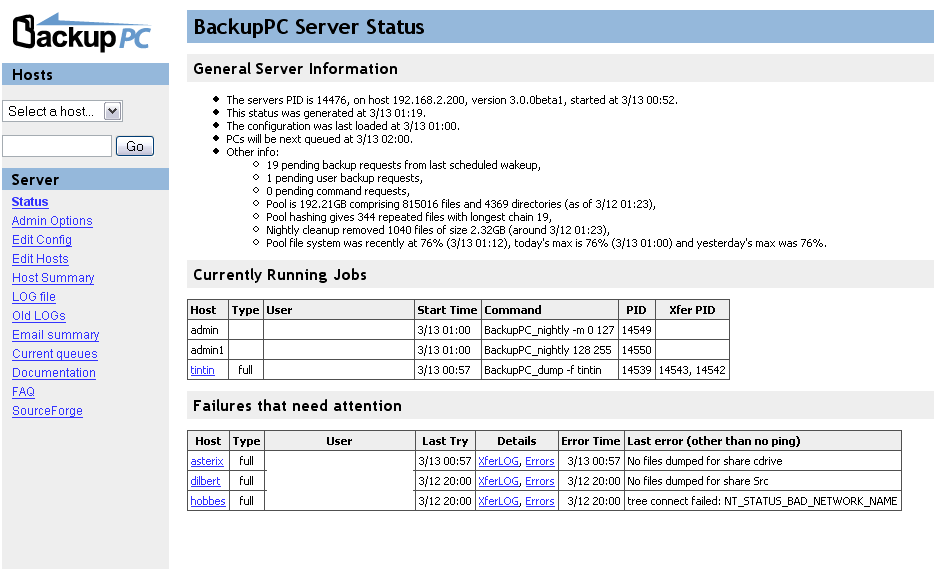
\includegraphics[width=13cm]{include/img/backuppc_server_status.png}
    \end{center}
    \caption{BackupPC Server Status}
    \label{fig:backuppc_server_status}
\end{figure}

\begin{figure}[H]
    \begin{center}
        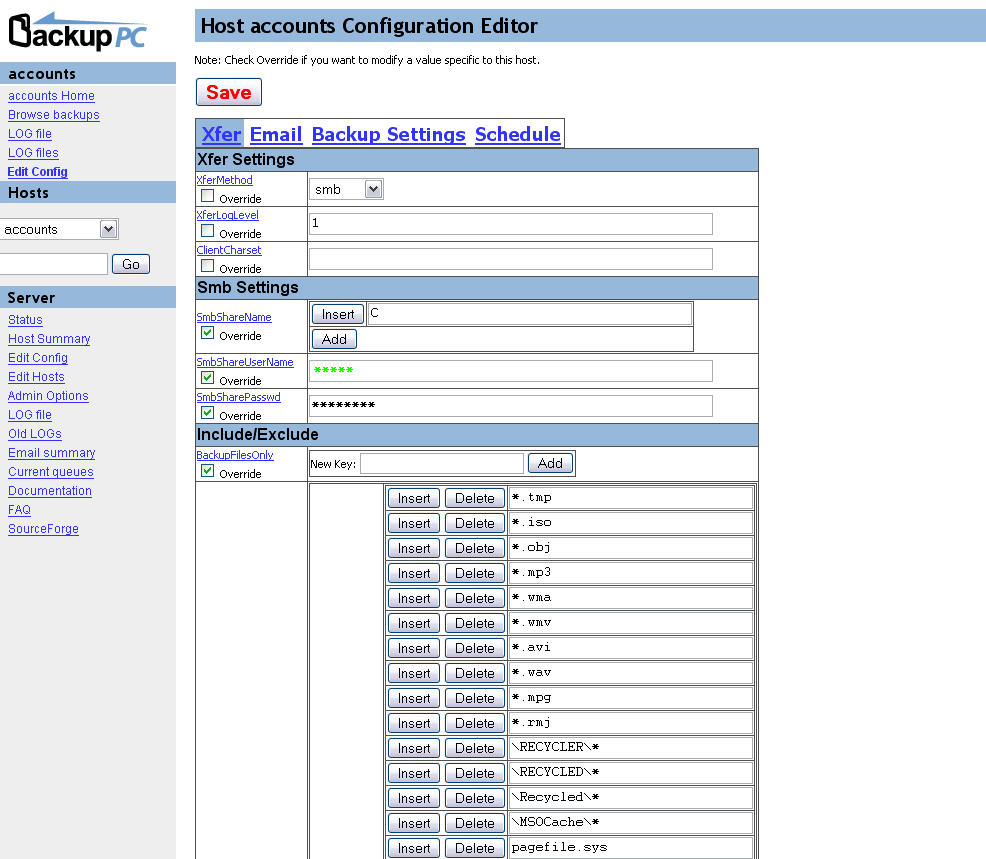
\includegraphics[width=13cm]{include/img/backuppc_edit_config.png}
    \end{center}
    \caption{Editar configuração}
    \label{fig:backuppc_edit_config.png}
\end{figure}


Informações adicionais podem ser obtidas em:\\ \begin{normalsize}\sffamily\href{http://backuppc.sourceforge.net/}{backuppc.sourceforge.net}\end{normalsize}
